\section{$N$+1-version Testing}\label{sec:idea}

In this section, we introduce the core concept of $N$+1-version testing with a
simple running example.  Then, we explain its overall structure consists of two
phases: a conformance test generation phase and a bug detection/localization
phase

\subsection{Main Idea}

The traditional $N$-version testing (or differential testing) utilizes the
cross-referencing Oracle, which is an assumption that any discrepency between
any program behaviors on the same input might be a potential bug.  Thus, it
compares the execution results of same inputs on different $N$ implementations
having same functionalities.  When an implementation provides a minority result
for a given input, it reports the implementation has a potential bug with the
input.

However, the $N$+1-version testing utilizes not only cross-referencing Oracle
from multiple implementations but also a mechanized specification.  It first
assumes that a mechanized specification as the Oracle and generates tests from
the specification.  Using the generated tests, it tests $N$ different
implementations and detects bugs.  Moreover, if most of implementations fail to
pass a test for the same reason, we are doubtful of the existence of bugs in
the specification.  Thus, $N$+1-version testing assumes that there exists a
specification bugs related to the test in this situation and localizes the bugs
in the specification based on the statistical information.


\subsection{Running Example}

\begin{figure}[t]
  \centering
  \begin{subfigure}[t]{0.48\textwidth}
    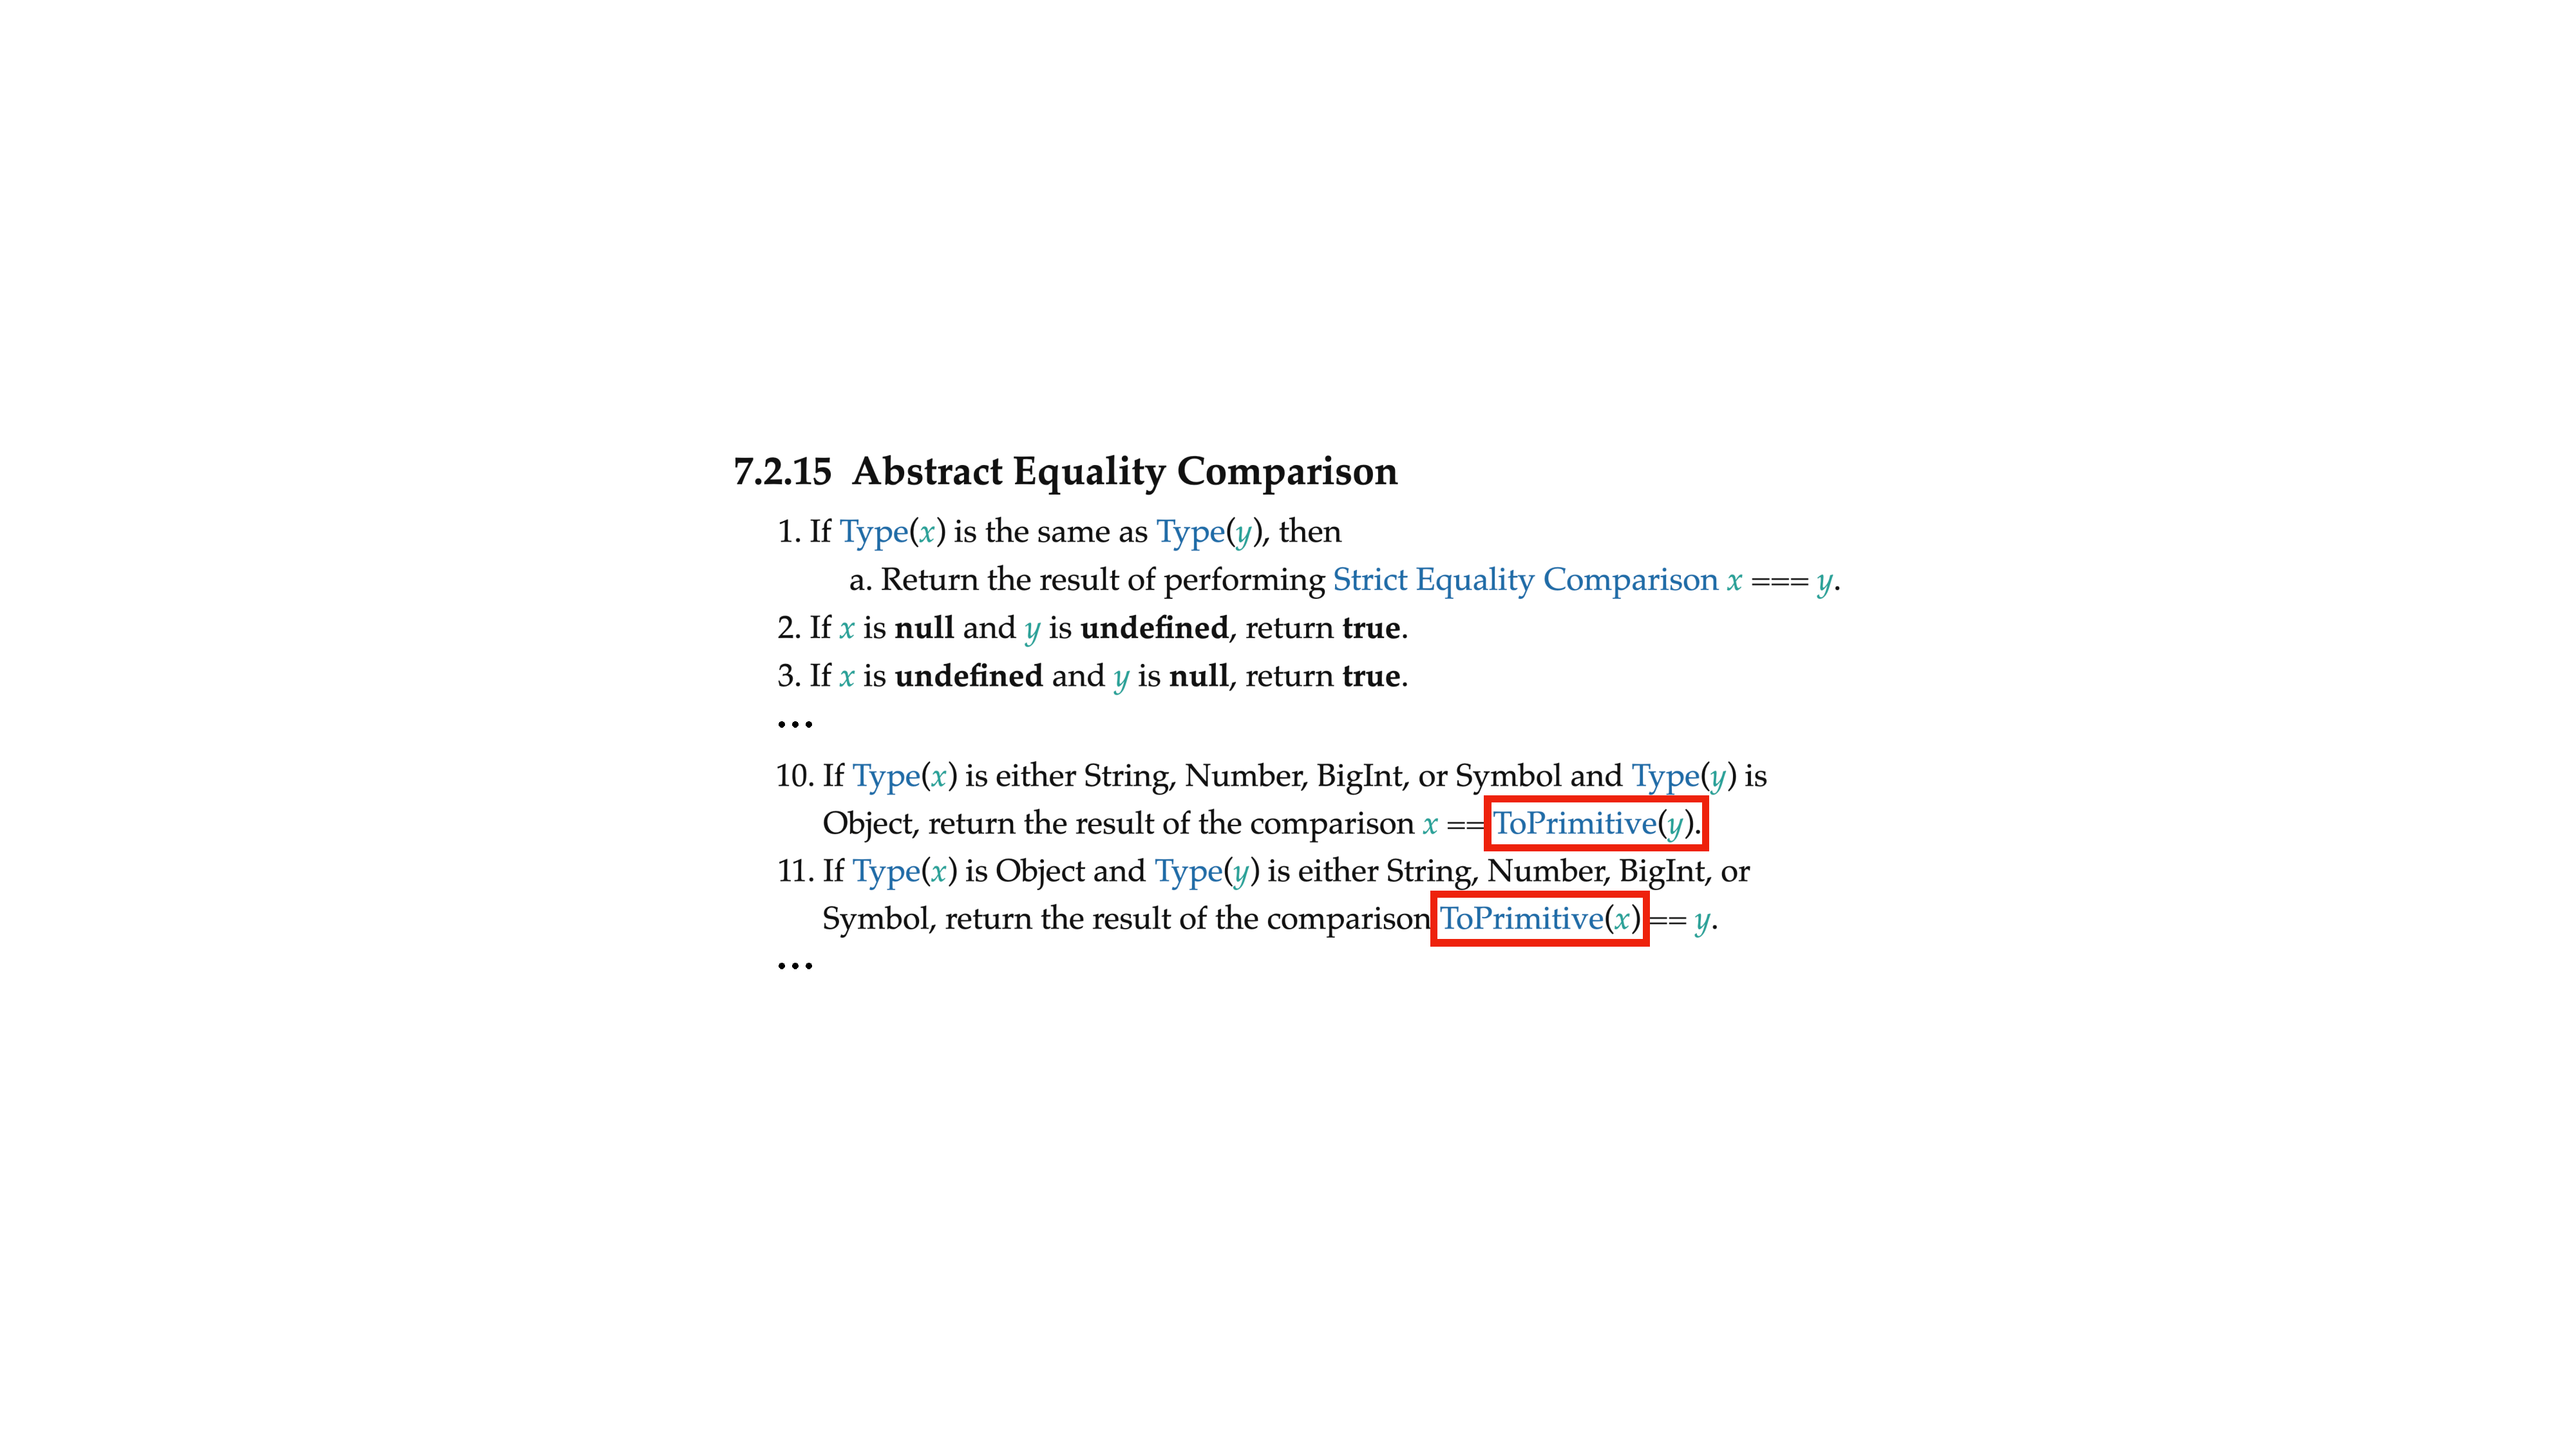
\includegraphics[width=\textwidth]{img/example-algo.pdf}
    \caption{The \textbf{Abstract Equality Comparison} abstract algorithm in
    ECMAScript 2020 (ES11)}
    \label{fig:example-algo}
  \end{subfigure}
  \begin{subfigure}[t]{0.43\textwidth}
    \begin{lstlisting}[style=myJSstyle]
var obj = { valueOf: () => { throw 'err'; } };
var result = 42 == obj;
// expected: throw an exception with 'err'
// ES11 semantics: result === false
    \end{lstlisting}
    \caption{An example JavaScript program}
    \label{fig:example-js}
  \end{subfigure}
  \begin{subfigure}[t]{0.45\textwidth}
    \begin{lstlisting}[style=myJSstyle]
try {
  var obj = { valueOf: () => { throw 'err'; } };
  var result = 42 == obj;
  assert(result === false);
} catch (e) {
  assert(false);
}
    \end{lstlisting}
    \caption{The assertion-injected JavaScript program}
    \label{fig:example-injected}
  \end{subfigure}
  \caption{A running example of $N$+1-version testing for JavaScript}
  \label{fig:example}
  \vspace*{-1em}
\end{figure}

\begin{figure*}[t]
  \centering
  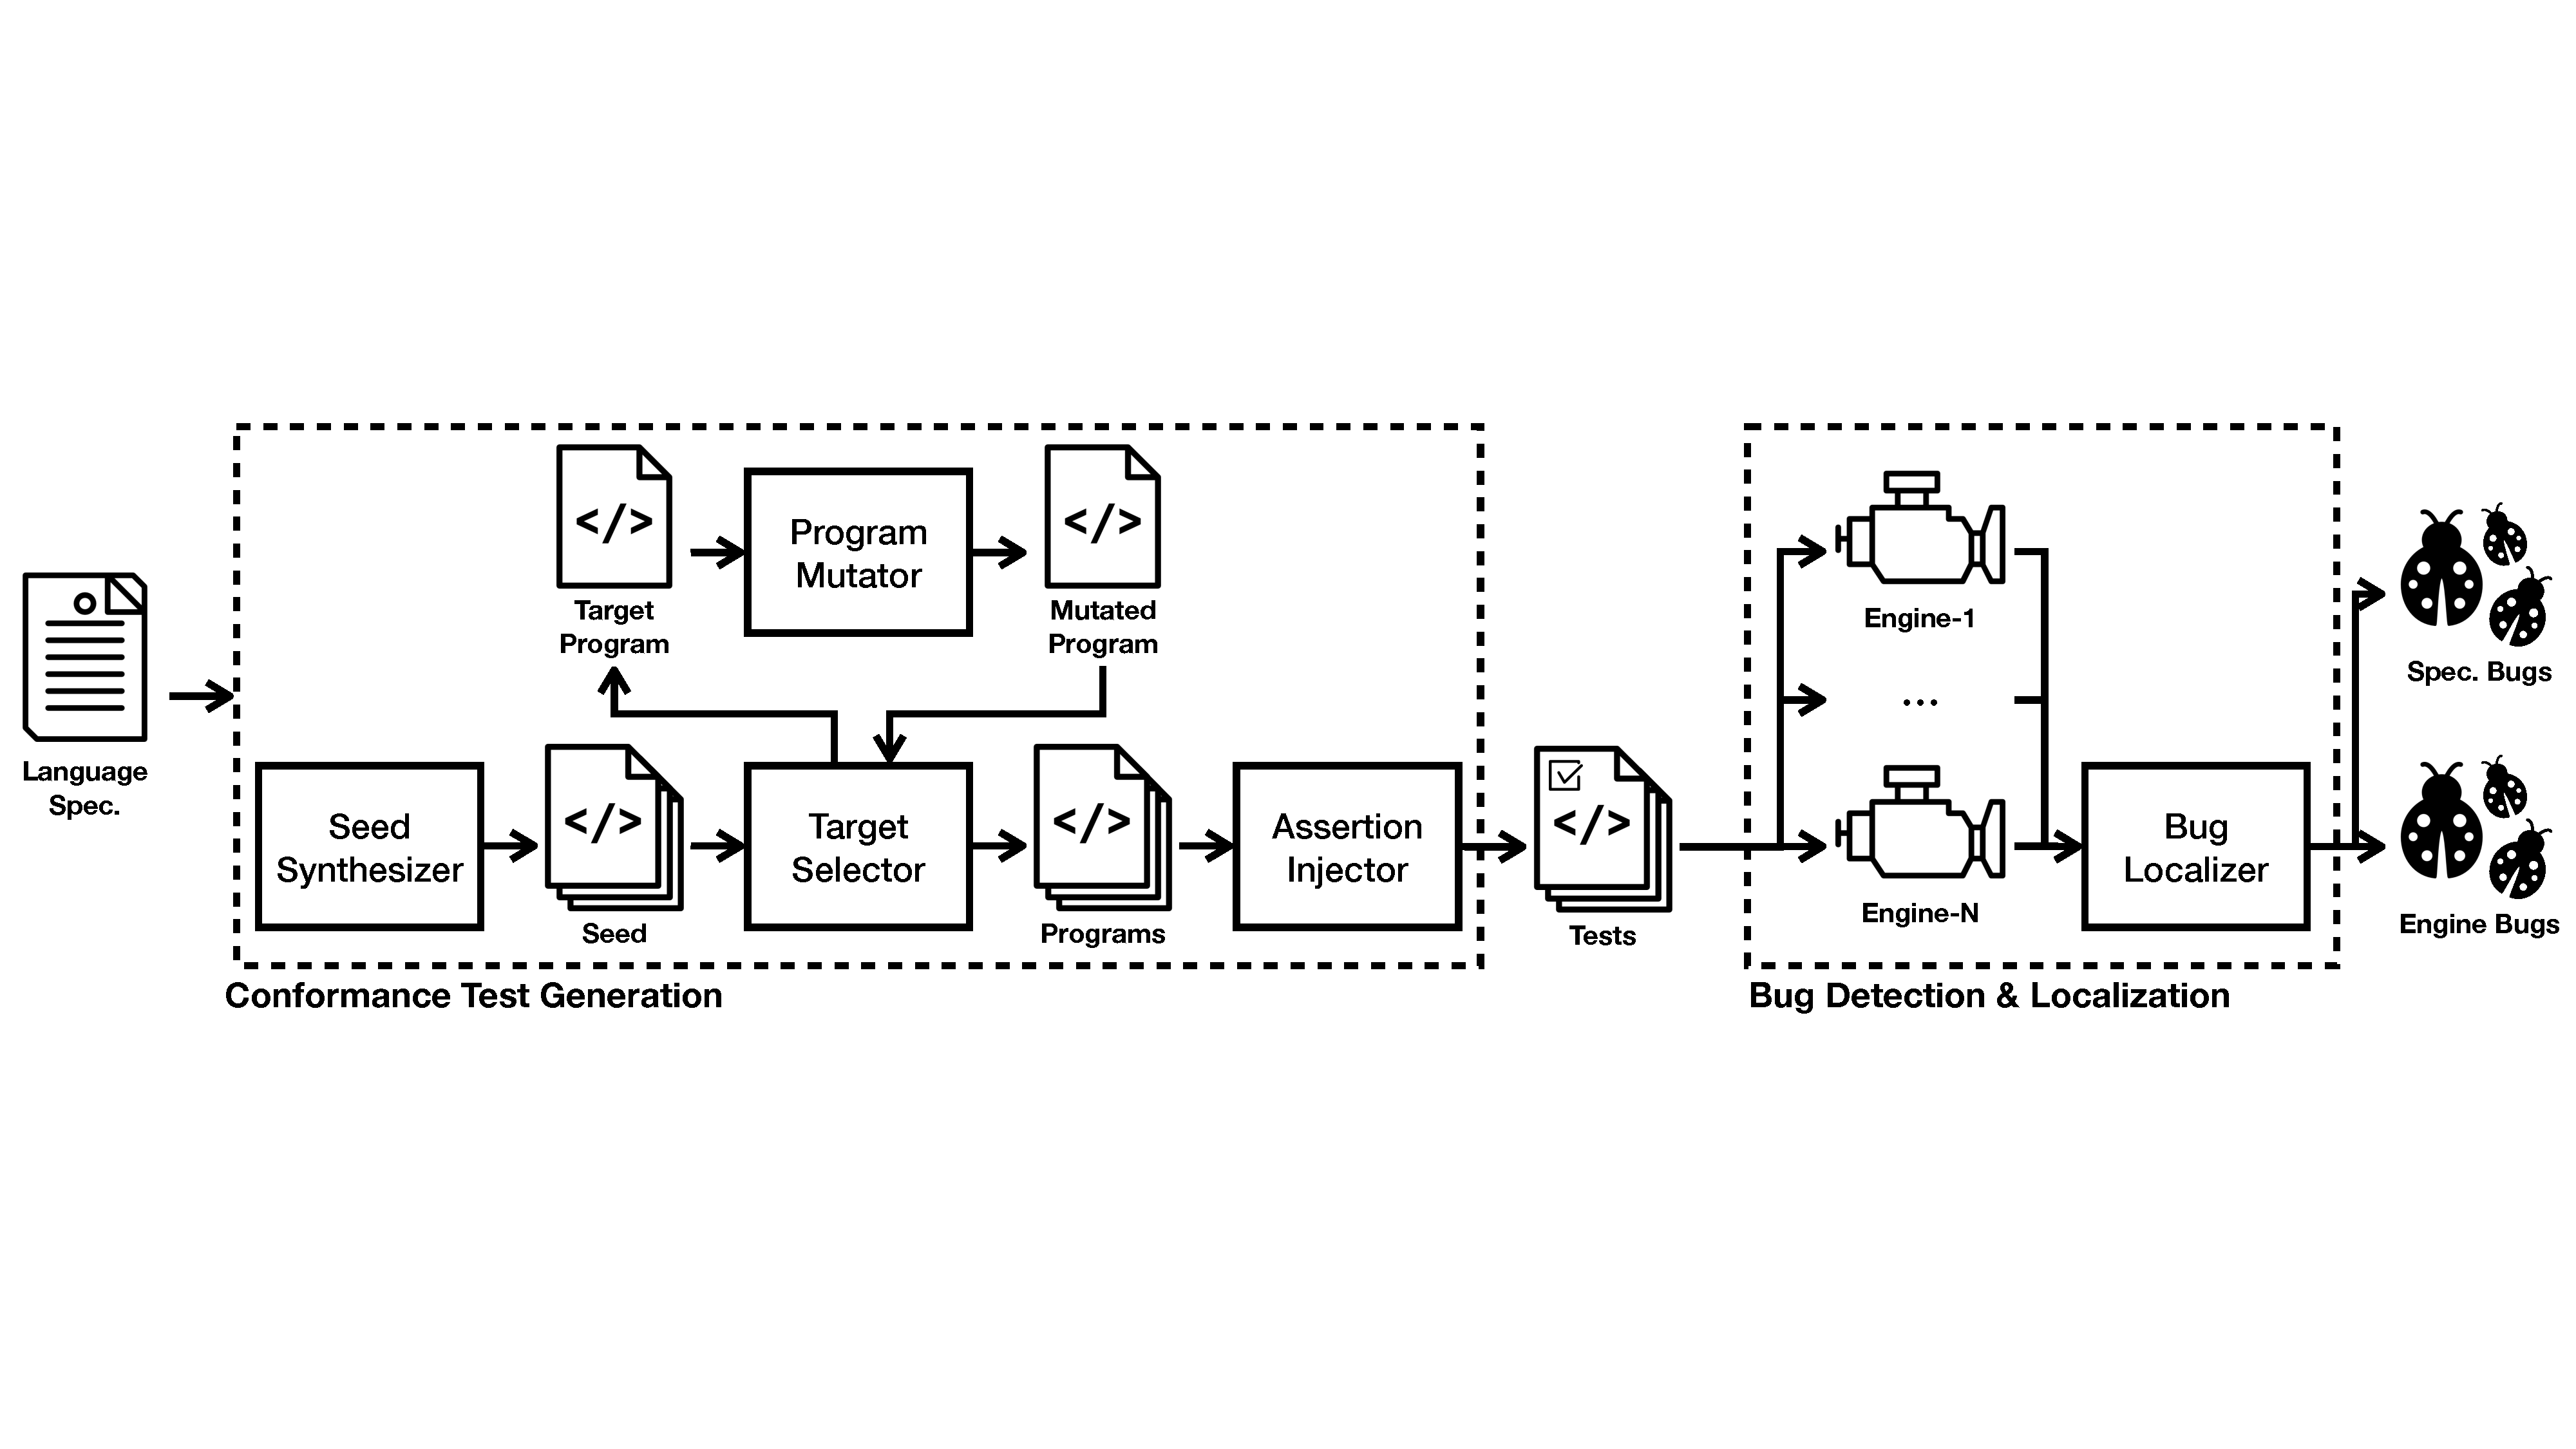
\includegraphics[width=0.95\textwidth]{img/n+1-version-testing.pdf}
  \caption{Overall structure of $N$+1-version testing for $N$ different
    implementations (engines) and a language specification.}
  \label{fig:overall}
  \vspace*{-1em}
\end{figure*}

Figure~\ref{fig:example} shows the running example of $N$+1-version for
JavaScript.  Figure~\ref{fig:example-algo} is a part of \textbf{Abstract Equality
Comparison} abstract algorithm in ECMAScript 2020 (ES11).  It describes the
semantics of non-strict equality comparison ($\code{==}$) between two JavaScript
values.  For example, $\code{null == undefined}$ is $\code{true}$ because of the
algorithm step 2.  According to step 10 and11, if a value has a String, Number,
BigInt, or Symbol type and the other value is an Object, the algorithm call the
\textbf{ToPrimitive} algorithm to convert the JavaScript object into a primitive
value and recursively call itself.  However, \textbf{ToPrimitive} algorithm
could return \textit{abrupt completion}.  ECMAScript uses completion values to
explain the runtime propagation of values and control flow such as behavior of
exceptions or $\code{break}$ statements.  When the type of a completion is not
$\code{normal}$ but one of $\code{break}$, $\code{continue}$, $\code{return}$,
and $\code{throw}$, the completion is called as an abrupt completion.  To handle
such abrupt completions, ECMAScript uses the question mark prefix (?) to check
and pass out the abrupt completions.  However, invocations of
\textbf{ToPrimitive} in step 10 and 11 do not use the question mark prefix (?).
Thus, it cannot pass out the exceptions introduced by \textbf{ToPrimitive} to
outisde.

For example, the JavaScript code in Figure~\ref{fig:example-js} causes the above
problem.  In the \textbf{Abstract Equality Comparison} algorithm, variables
\textit{x} and \textit{y} denote $\code{42}$ and an object whose property
$\code{valueOf}$ points to an arrow function that throws an error.  In step 10,
the object is passed to the \textbf{ToPrimitive} function and it returns an
abrupt completion because the function stored in $\code{valueOf}$ throws an
error.  However, the specification silently ignores the abrupt completion and
returns $\code{false}$ as the result of comparison.  Based on the semantics
described in the specification, we could inject assertions to check the code
does not throw any erros as described in Figure~\ref{fig:example-injected}.
However, most of modern JavaScript engines throw an error with a string
$\code{'err'}$.  Using this information, we know that there exists a potential
specification bug with the JavaScript code.  Moreover, we can localize the
detected bug using the statistical information. Among bunch of conformance
tests, most of tests that go through steps 10 and 11 in the algorithm would be
fail in most of JavaScript engines.  It gives us the information that the bug
exists in the steps 10 and 11 of \textbf{Abstract Equality Comparison} with high
probability.


\subsection{Overall Structure}

Figure~\ref{fig:overall} depicts the overall structure of $N$+1-verison testing
for $N$ different engines and a language specification.  It consists of two
phases: a conformance test generation phase and a bug detection/localization
phase.  Based on a given language specification, it automatically generates
conformance tests that reflect the language syntax and semantics described in
the specification.  Then, it detects and localizes engine or specification bugs
via results of the generated tests on $N$ different engines.  Now, we introduce
each module in $N$+1-version testing and explain its functionalities.
\newline

\subsubsection{Seed Synthesizer}
At the first step, \textsf{Seed Synthesizer} synthesizes initial seed programs
based on the language syntax.  Its main goal is to synthesize 1) few number of
2) small sized programs 3) that cover possible cases in syntax rules as many as
possible.
\newline

\subsubsection{Target Selector}
For a given program pool, it selects a target program in the program pool
depending on the semantics coverage of program pool.  The initial program pool
is the seed programs generated by \textsf{Seed Synthesizer}. The program pool
will grow by adding a new program mutated by \textsf{Program Mutator} from
the selected target program.  When specific criteria are satisfied,
\textsf{Target Selector} stops to select target program and gives programs in
the current program pool as the result.
\newline

\subsubsection{Program Mutator}
The main goal of \textsf{Program Mutator} is to generate a new program by
mutating a given target program in order to increase the semantics coverage.
If it fails to generate a new program to increase semantics coverage,
\textsf{Target Selector} selects a new target program again and repeat this
process less than the pre-defined maximum iteration number.
\newline

\subsubsection{Assertion Injector}
It modifies given programs to conformance tests by injecting appropriate
assertions reflecting the semantics described in the specification.
\textsf{Assertion Injector} executes each program under the mechanized
specification and obtains the final state of the execution.  Based on the final
state, it automatically inject assertions to the program.
\newline

\subsubsection{Bug Localizer}
First, it executes the given conformance tests on $N$ different engines and
collects the test results.  For each test, if minor engines fail,
it reports the potential bugs in the engines fail the test.  Otherwise, it
reports the potential bugs in the specification.  It utilizes \textit{coverage
based statistical fault localization} (CBSFL)~\cite{fault-local}.  It uses coverage
information of tests to rank the statements from most suspicious to least
suspicious ones.

% 참고 https://hackthology.com/how-to-evaluate-statistical-fault-localization.html
